\subsection{Example}\label{sec:sample-example}

The set-based approach to solving inverse problems can lead to errors in approximating measures, particularly around the boundaries of the solution set.
By contrast, the sample-based approach we introduced above more accurately approximates a uniform density over a subset of the initial parameter space at a given sample size $\nsamps$.
The reason for this is that the approach has a different source of error, involving estimating to push forward of the initial density.
The sample-based approach does not rely on a Voronoi-cell approximation of contour events, and instead assigns probability to random samples drawn from an initial density.

We are interested in studying how our ability to estimate a uniform density is impacted by the number of samples drawn from the initial density.
We form an inverse problem with the identity map an standard uniform initial densities, with observed densities being uniform over $[0.4, 0.6]^2$, representing a hundred-fold reduction in uncertainty when the problem is solved

We solve the same problem as in the set-valued example \ref{sec:set-example}, but use a uniform initial density in place of a uniform ansatz.
We sample $N=1E2$, $1E3$ and $1E4$ samples from the initial density and use Gaussian kernel density estimation to approximate the denominator in Eq [TK - eq], and show the resulting updated densities in Figure~\ref{fig:ex:identity_sampling_1E2} and \ref{fig:ex:identity_sampling_1E3_1E4} alongside the analytical solution.

The jagged edges of the shapes that we saw in \ref{fig:ex:identity_set_1E3_1E4} are replaced by unambiguous squares.
The relative probability that is assigned within the support is also more uniform, visually represented by the uniformity of color in the density plot.

\begin{figure}
\begin{minipage}{.975\textwidth}
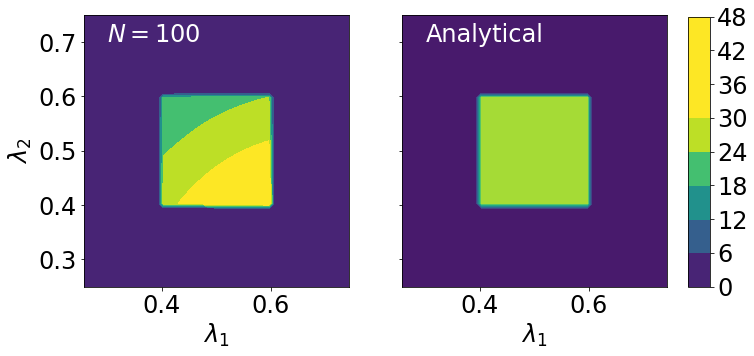
\includegraphics[width=\linewidth]{./examples/identity/samp/N100_N100-vs-Analytical_N100.png}
\end{minipage}
\caption{
(Left): $\nsamps=100$ were used to construct the predicted distribution $\predicted$.
(Right): By specifying an analytical $\predicted$, the effect of using $\nsamps$ to approximate a pushforward distribution disappears. The problem can be fully specified in BET without any random sampling.
}
\label{fig:ex:identity_sampling_1E2}
\end{figure}

\begin{figure}
\begin{minipage}{.975\textwidth}
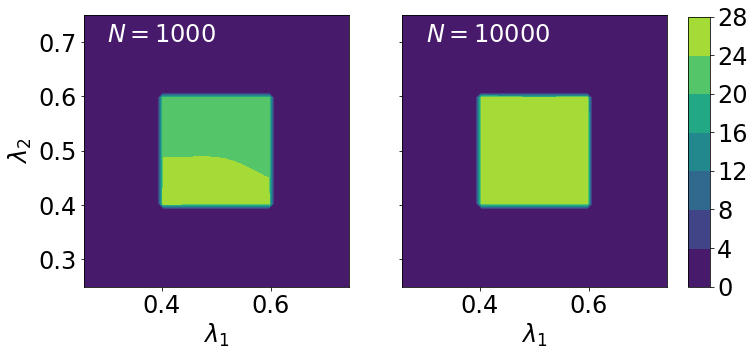
\includegraphics[width=\linewidth]{./examples/identity/samp/N1000_N1000-vs-N10000_N10000.png}
\end{minipage}
\caption{
$\nsamps=1,000$ (left) and $\nsamps=10,000$(right) were used to construct the predicted distribution $\predicted$.
There is no signficant error in estimating the support of the distribution, only the density approximation itself.
}
\label{fig:ex:identity_sampling_1E3_1E4}
\end{figure}


The sample-based method trades one source of accuracy for another.
The sample-based method provides a compelling alternative to be set-based method when estimating boundaries of a set (which represents an equivalent class of solutions), is important.
When few model evaluations are available and the observed distribution is non-uniform, the lack of need to use nearest-neighbor sampling (discretizing with $\ndiscs$), also provides a benefit.
However, we know that this is not without its pitfalls, as density estimation in high dimensions can become prohibitively prone to error \cite{Silverman}.
